\chapter{Nestor example 2}
%

% - Purpose & Problem description:
%     These first two parts give reader short details about the test case,
%     the physical phenomena involved and specify how the numerical solution will be validated
%
\section{Purpose}
%
Second test example for Nestor performing the action:

\texttt{ActionType = Dump\_by\_time}
%
\section{Description of the problem}
%
This example performs the dumping of supply material with the dumping being optionally planar or non-planar.
Two dumping areas are defined by polygons which are defined in file \texttt{\_DigPolys.dat}. They are located in the larger widening between 615,5 and 766,5 m (see Figure~\ref{ini}).
The area of each polygon is 1173 m$^2$ and each ploygon covers a hollow in the bottom. The deepest points in the hollows are 3 m below the plain bottom.
The supply material is composed of the two finest and the two most coarse fractions of the bed sediment.


Using the option DumpPlanar = FALSE 586.5 m$^3$ supply material will be dumped in the polygon named \texttt{401\_hollow1\_1173m**2} over a time period of 120 s. As result the all nodes in the area will elevate about the same value. In this case about 0.5 m.

Using the option DumpPlanar = TRUE 586.5 m$^3$ supply material will be dumped in the polygon named \texttt{402\_hollow2\_1173m**2} over a time period of 120 s. As result the hollow will be filled up starting from the deepest points in the area until the whole supply material is used. Thus only the deeper nodes will be changed.
At the end of the dumping the plain spanned through the changed nodes is parallel to the plain  defined in the reference level file \texttt{\_DigRefLevel.dat}

Due to the mixing processes of the Hirano layer model, all nodes which changed the bottom elevation, will have a modified sediment distribution.


Convention for naming polygons: The polygon name must start with an integer between 100 and 999. Any text after that is treated as a comment to  help the user.
Internally only the number is used to identify the polygon.


% - Physical parameters:
%     This part specifies the geometry, details all the physical parameters
%     used to describe both porous media (soil model in particularly) and
%     solute characteristics (dispersion/diffusion coefficients, soil <=> pollutant interactions...)
%
%
\subsection{Physical parameters}
%
The simulation is set up with ten grain classes.
The bottom is discretised with three layers. A constant active layer (0.1 m), an underlying stratum (0.1 m) and a third layer up to the rigid bed (9.8m).

The Meyer-Peter Mueller (MPM) transport formula is used but the MPM parameter is set to zero to avoid sediment transport. Thus all bottom changes are a result of the two dumping processes.
% - Geometry and Mesh:
%     This part describes the mesh used in the computation
%
%
\subsection{Geometry and Mesh}
%
A 1000 m long flume with three widening parts has been chosen as test geometry (see Figure~\ref{ini}).
The width of the flume is 10 m and increases up to 30 m in the widening parts.
Two of the widening parts are 100 m long and the third is 200 m long.
The initial bottom has a continuous slope of 0,9 ppm with two hollows in the third widening.
The node area for every node is 1 m$^2$ in order to calculate and check dredging and dumping volumes easily.

The mesh consists of 18411 nodes and 34800 elements.

\begin{figure} [!h]
\centering
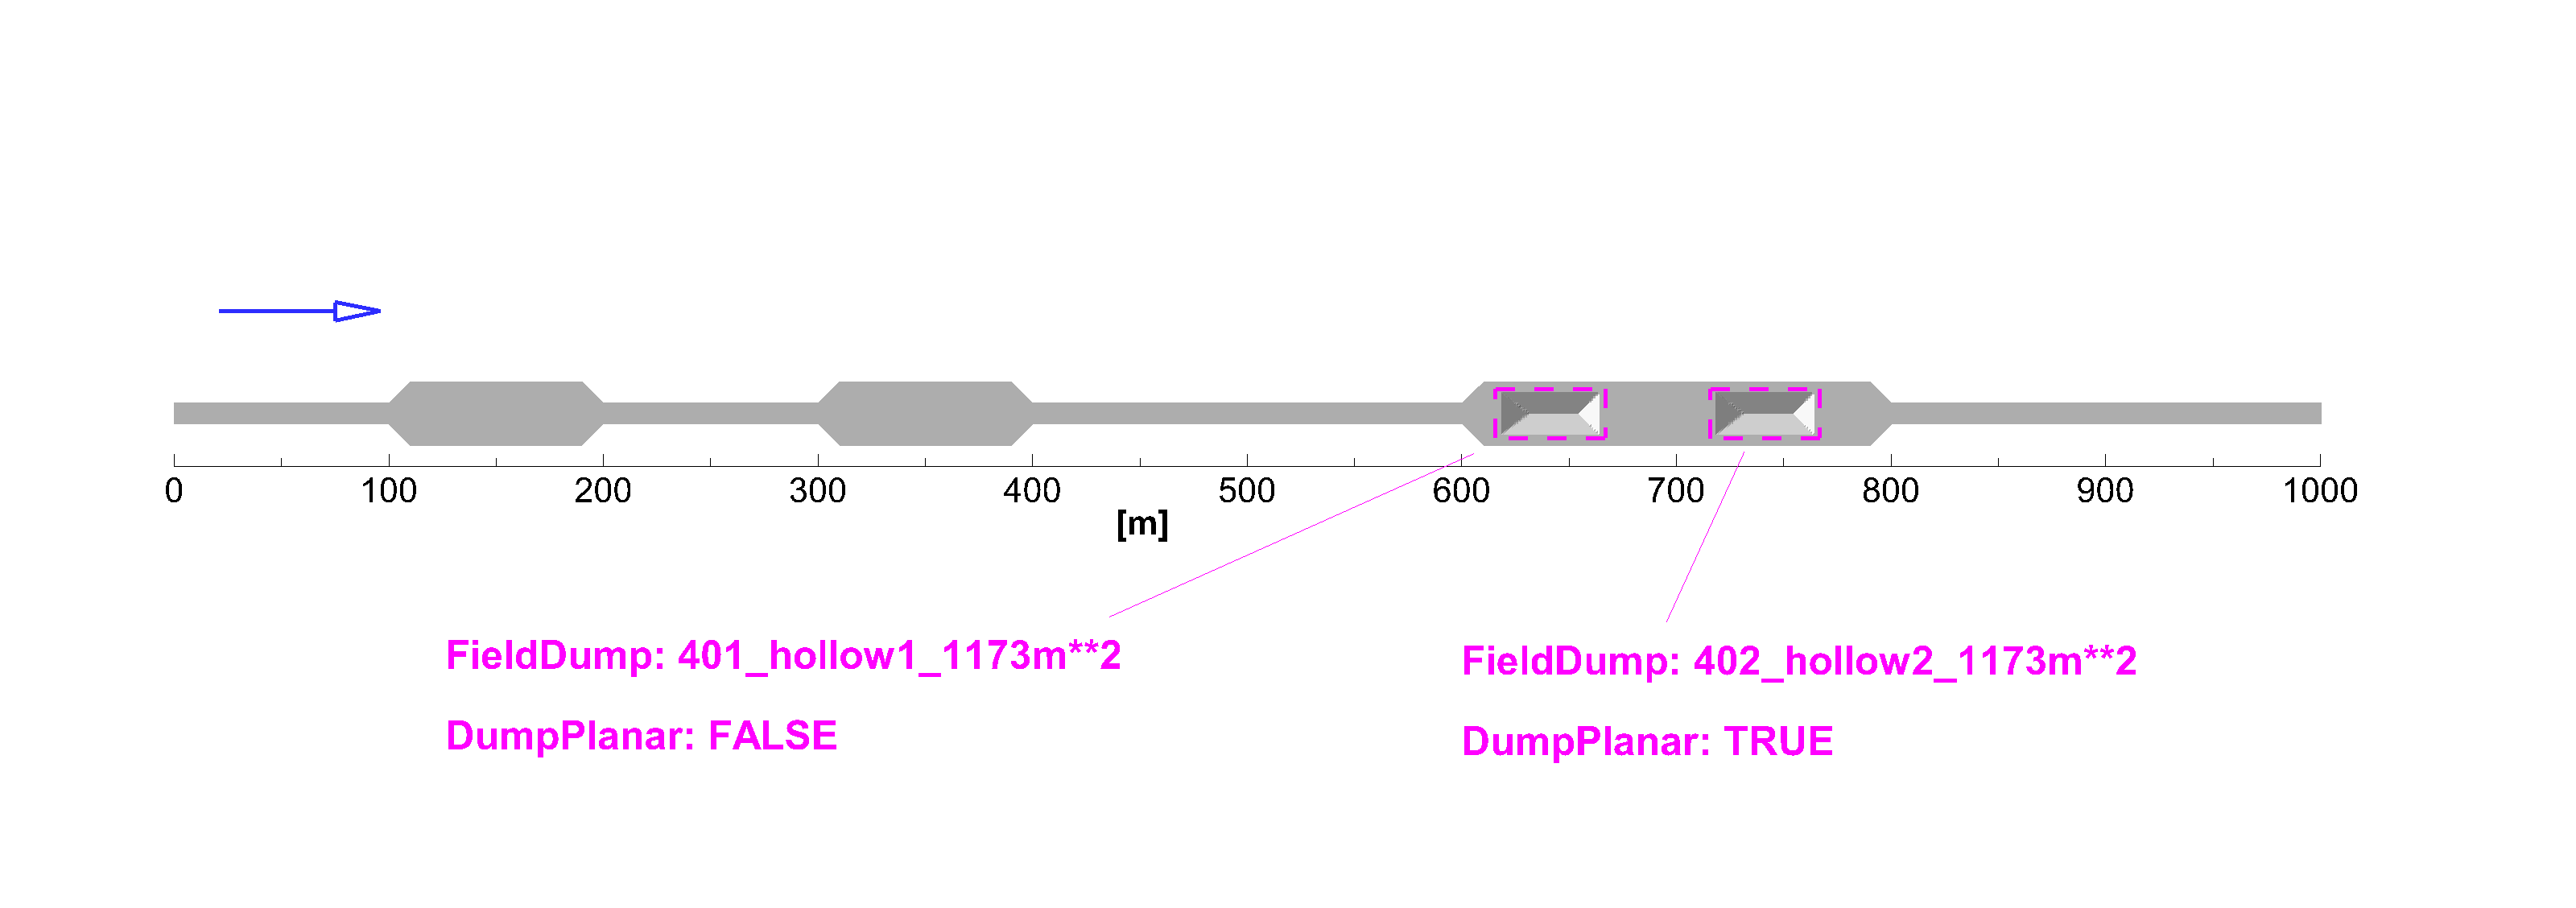
\includegraphics[scale=0.14]{result000.png}
 \caption{Geometry of the test flume with three widening parts the two hollows and the two polygons}\label{ini}
\end{figure}


% - Initial and boundary conditions:
%     This part details both initial and boundary conditions used to simulate the case
%
%
\subsection{Initial and Boundary Conditions}
%
Steady state boundary conditions:
\begin{itemize}
\item{Discharge at the inlet = 20 m$^3$/s}
\item Water depth at outlet = 1 m
\item Sedimentological equilibrium at the inlet (zF is constant, QS will be calculated)
\end{itemize}
Fully developed flow from a previous simulation is used as initial conditions.

The total simulation period is 150 s with a time step of 1 s.
% - Numerical parameters:
%     This part is used to specify the numerical parameters used
%     (adaptive time step, mass-lumping when necessary...)
%
%
\subsection{Numerical parameters}
%
% - Results:
%     We comment in this part the numerical results against the reference ones,
%     giving understanding keys and making assumptions when necessary.
%
%
\section{Results}
%
Figure~\ref{result50} shows the evolution after 0s, 70s and 150s. The dumping process finished at 122s.

% Here is an example of how to include the graph generated by validateTELEMAC.py
% They should be in test_case/img
\begin{figure} [!h]
\centering
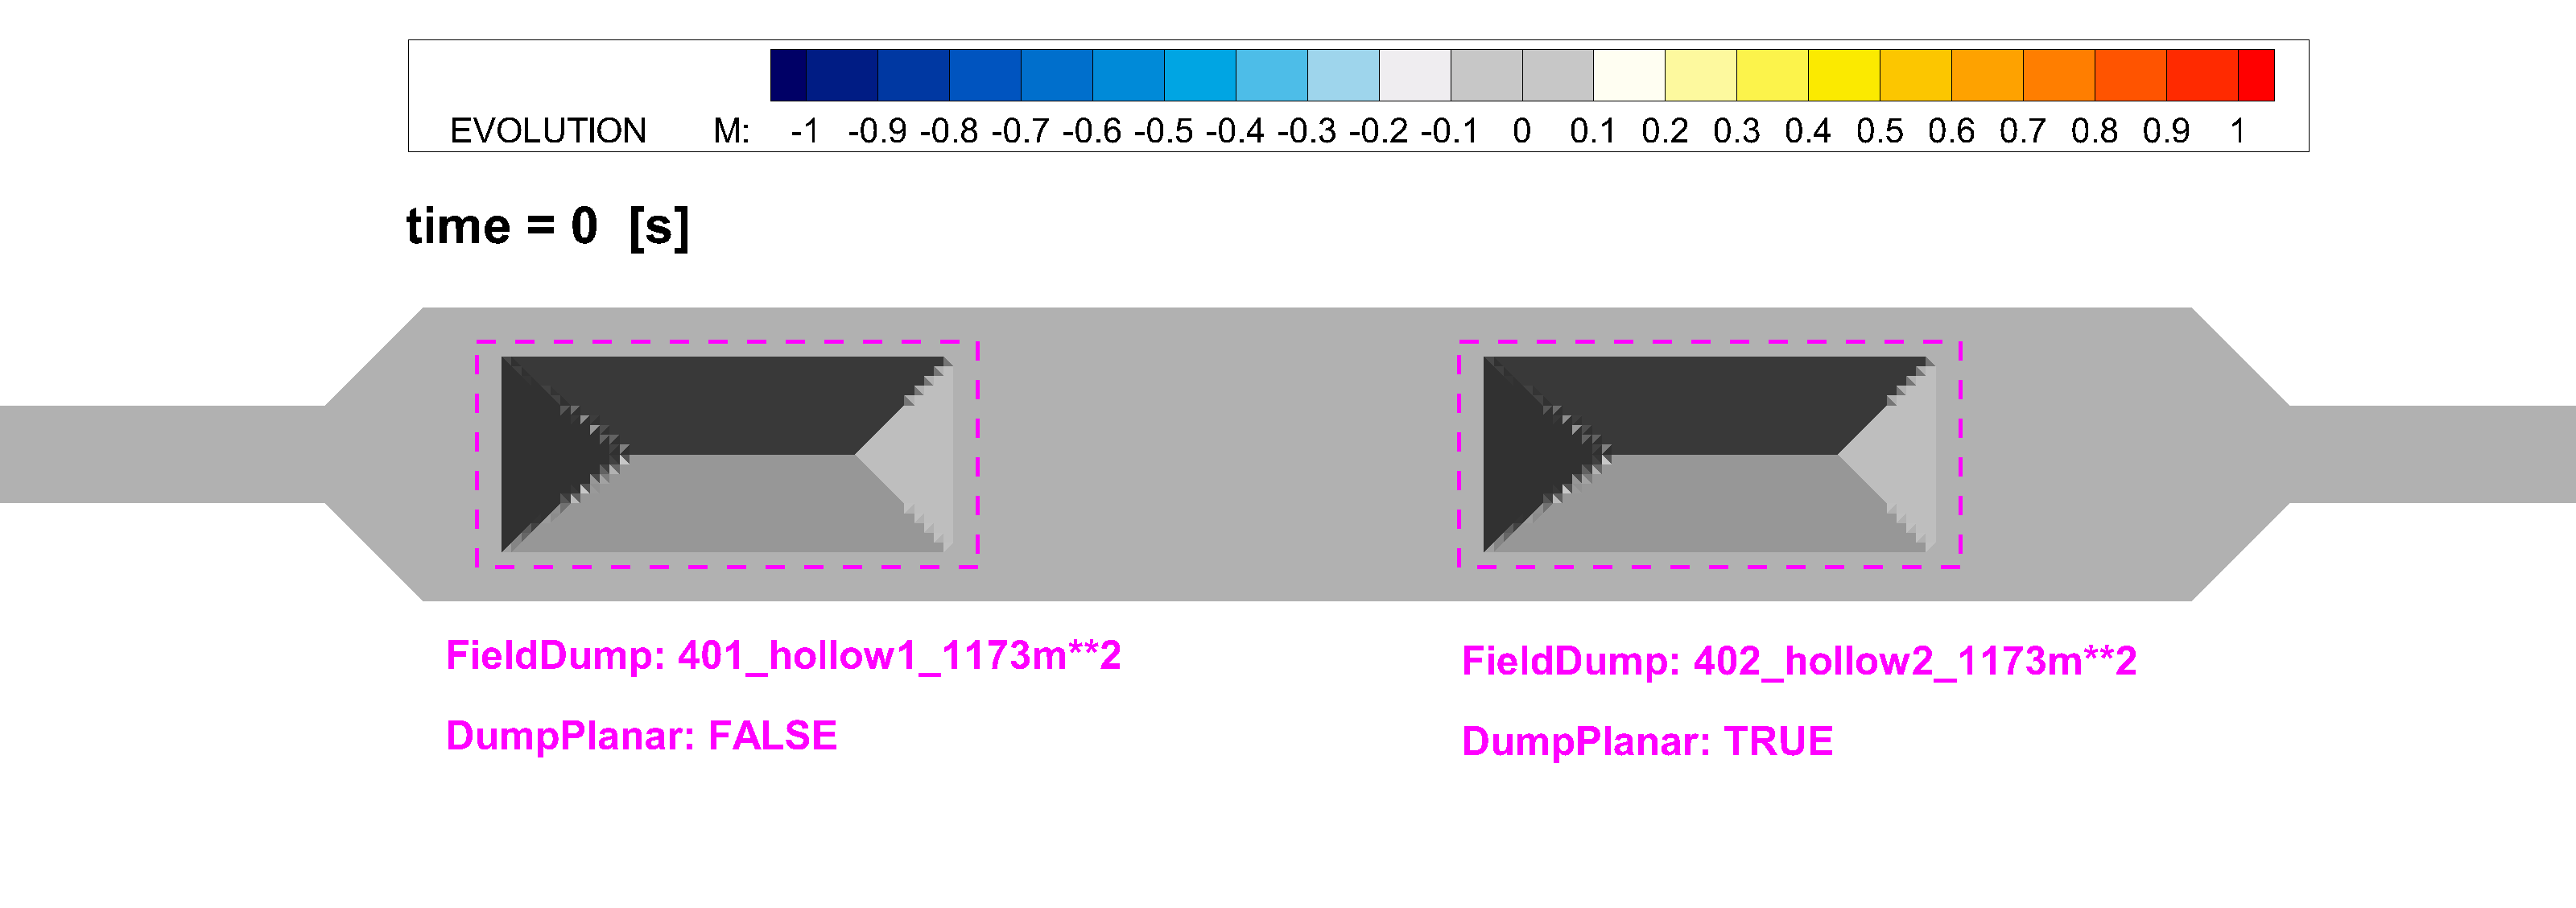
\includegraphics[scale=0.14]{result000_zoom.png}
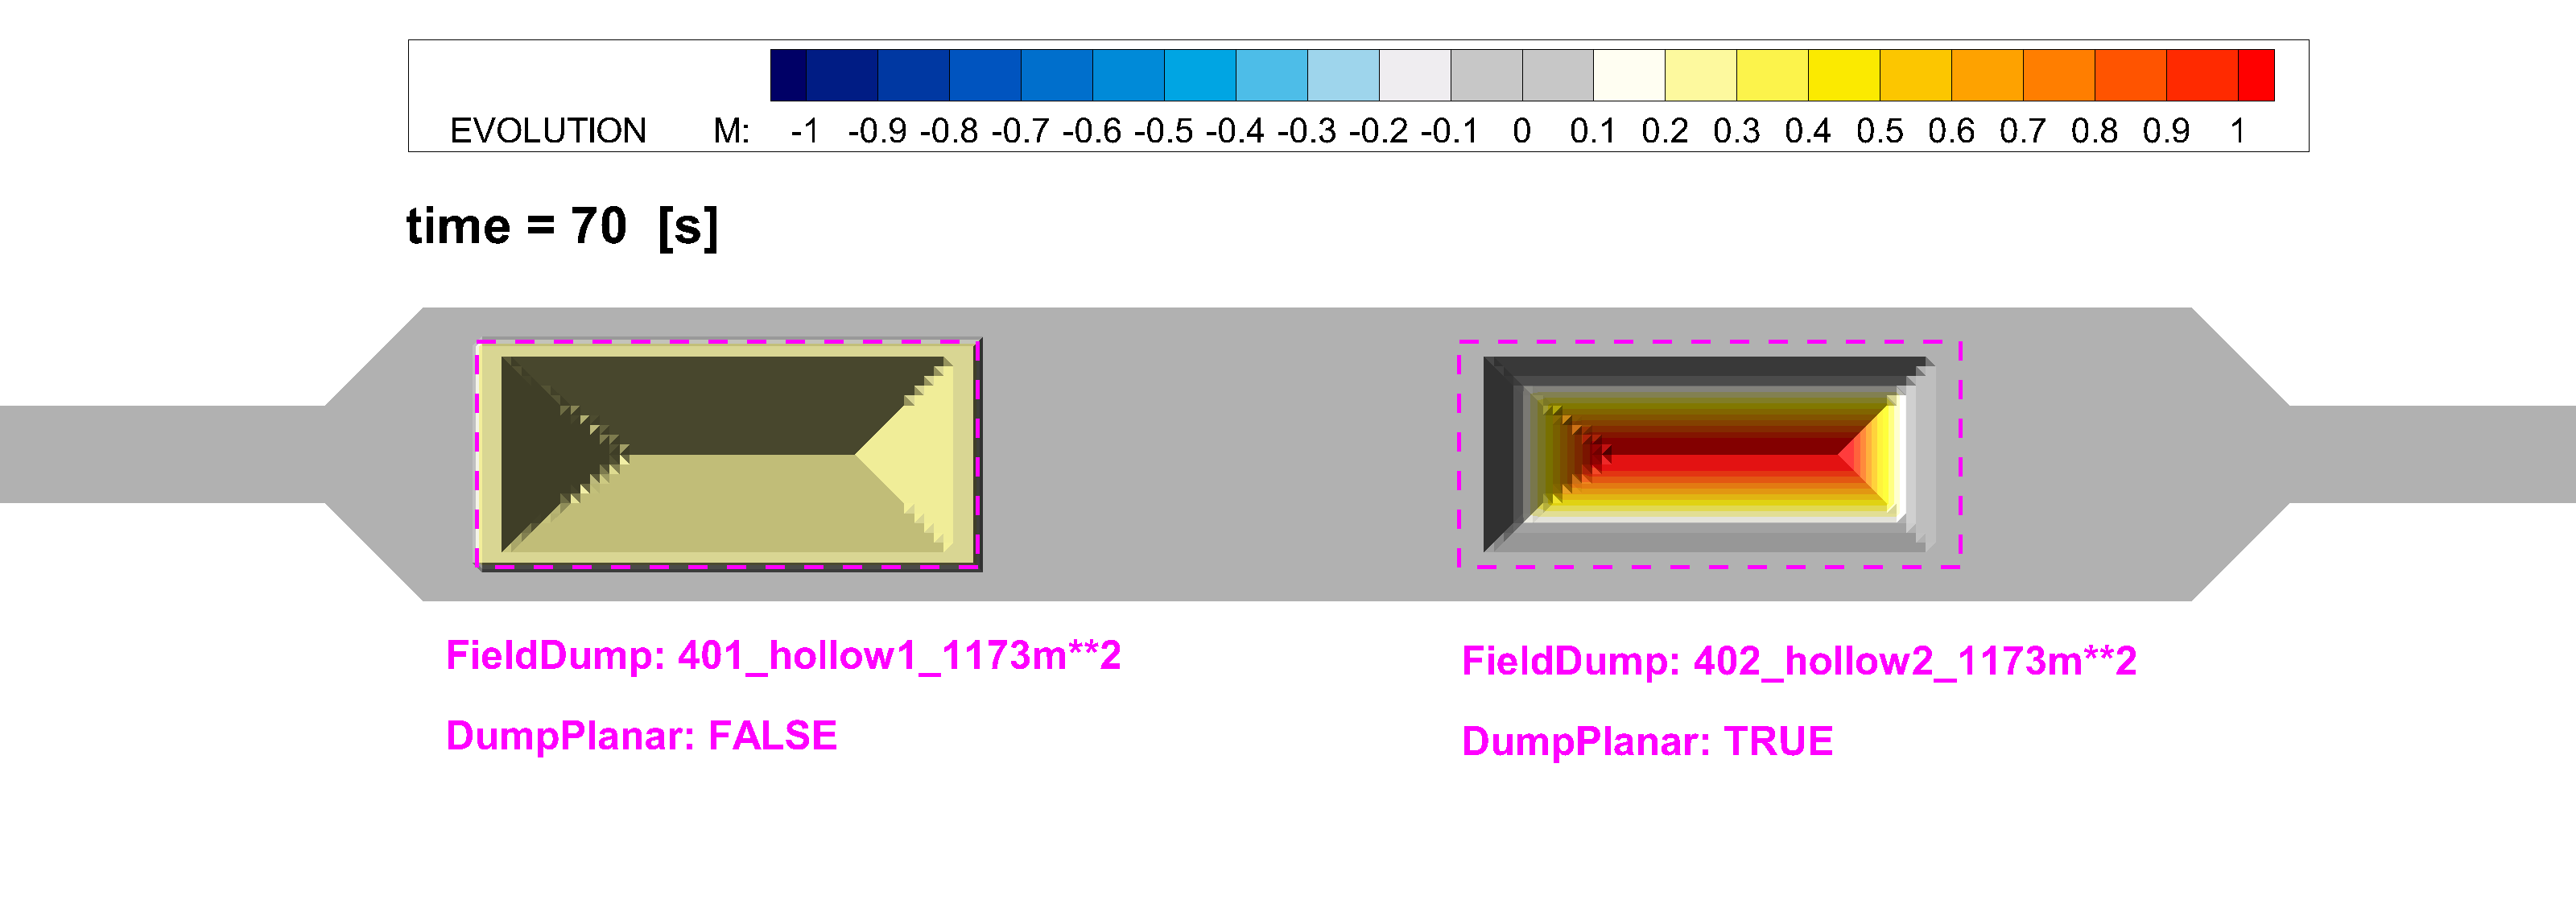
\includegraphics[scale=0.14]{result070_zoom.png}
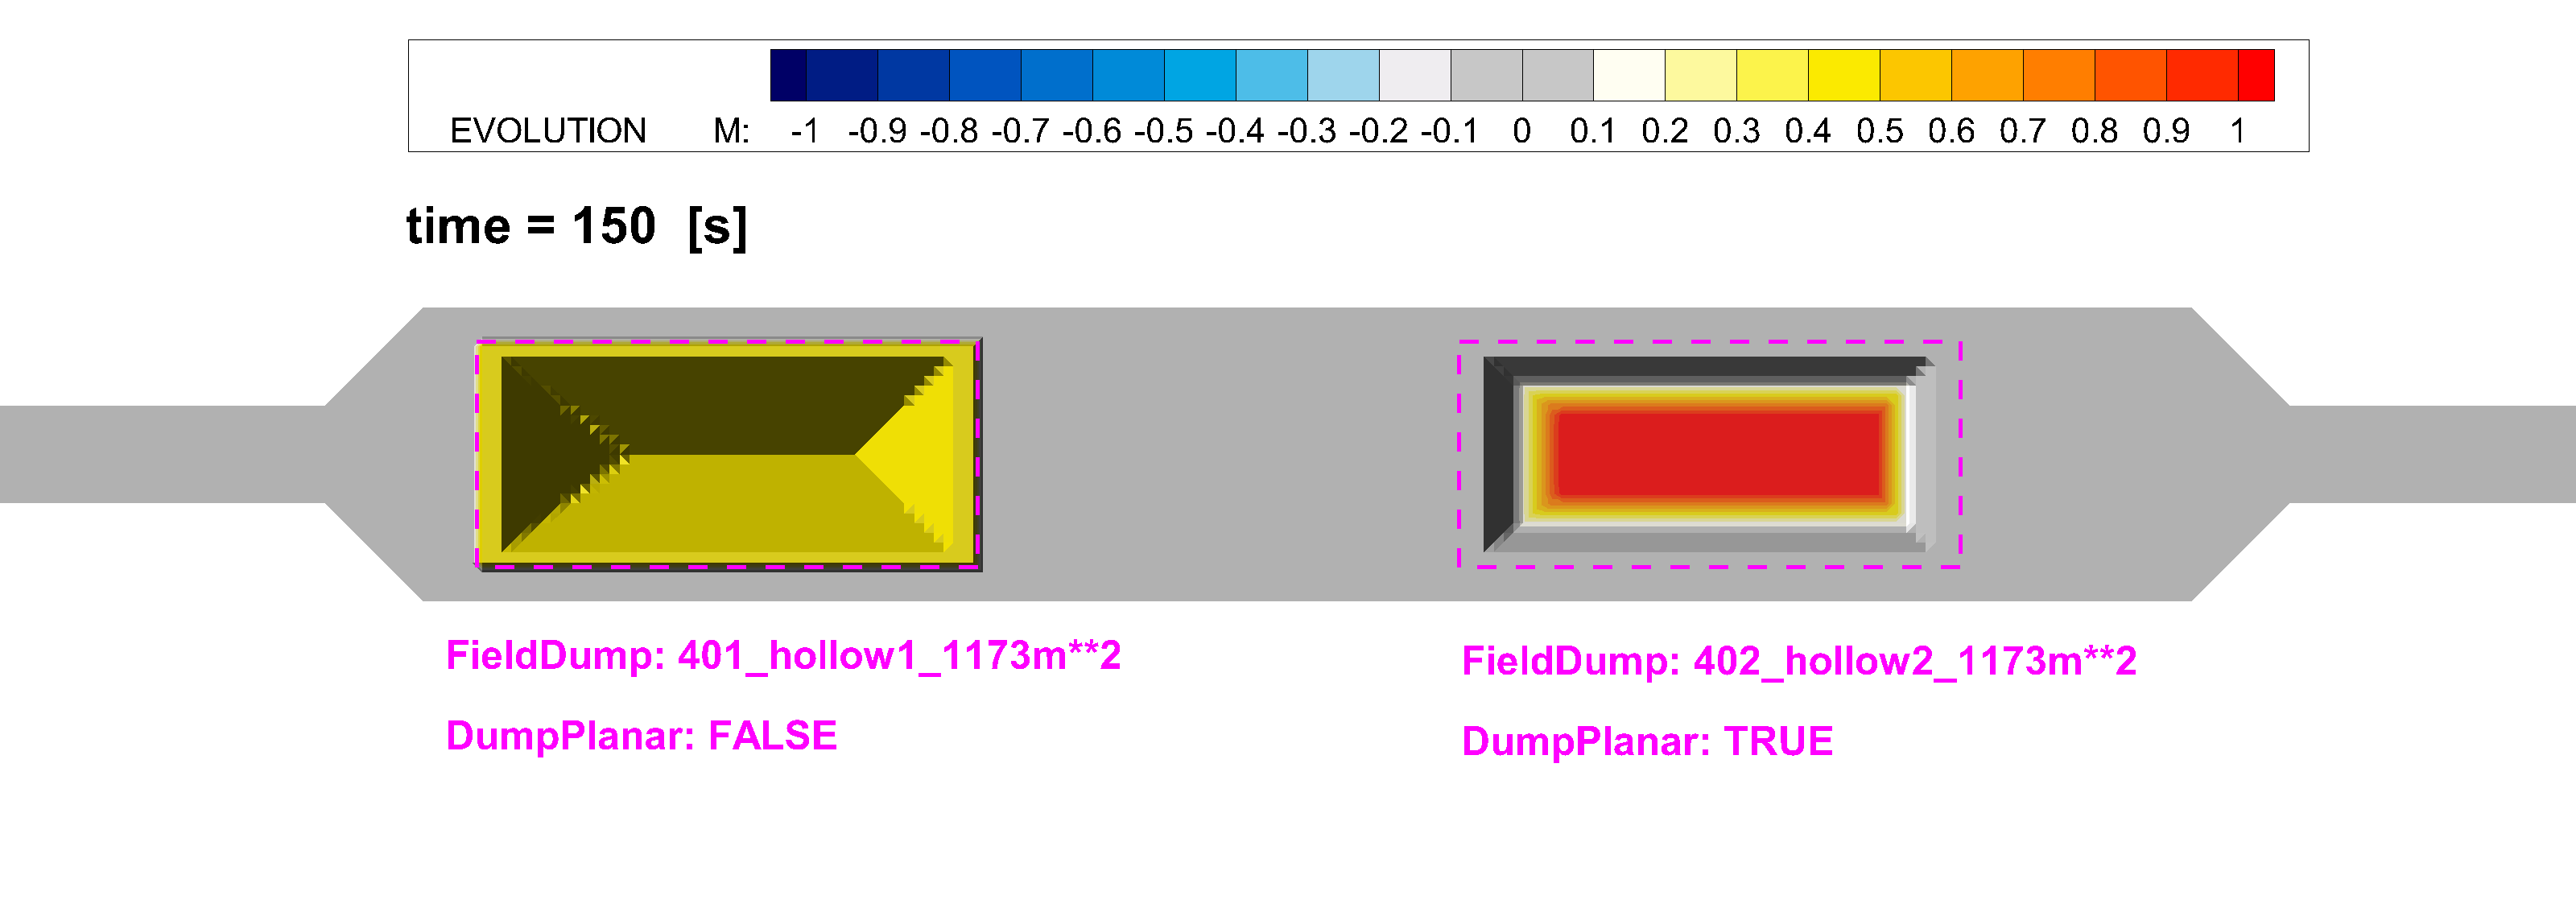
\includegraphics[scale=0.14]{result150_zoom.png}
\caption{Simulated evolution after 0, 70 and 150 s.}\label{result50}
\end{figure}

Figure~\ref{result3D} shows the evolution after 0s and 150s as 3D view.
\begin{figure} [!h]
\centering
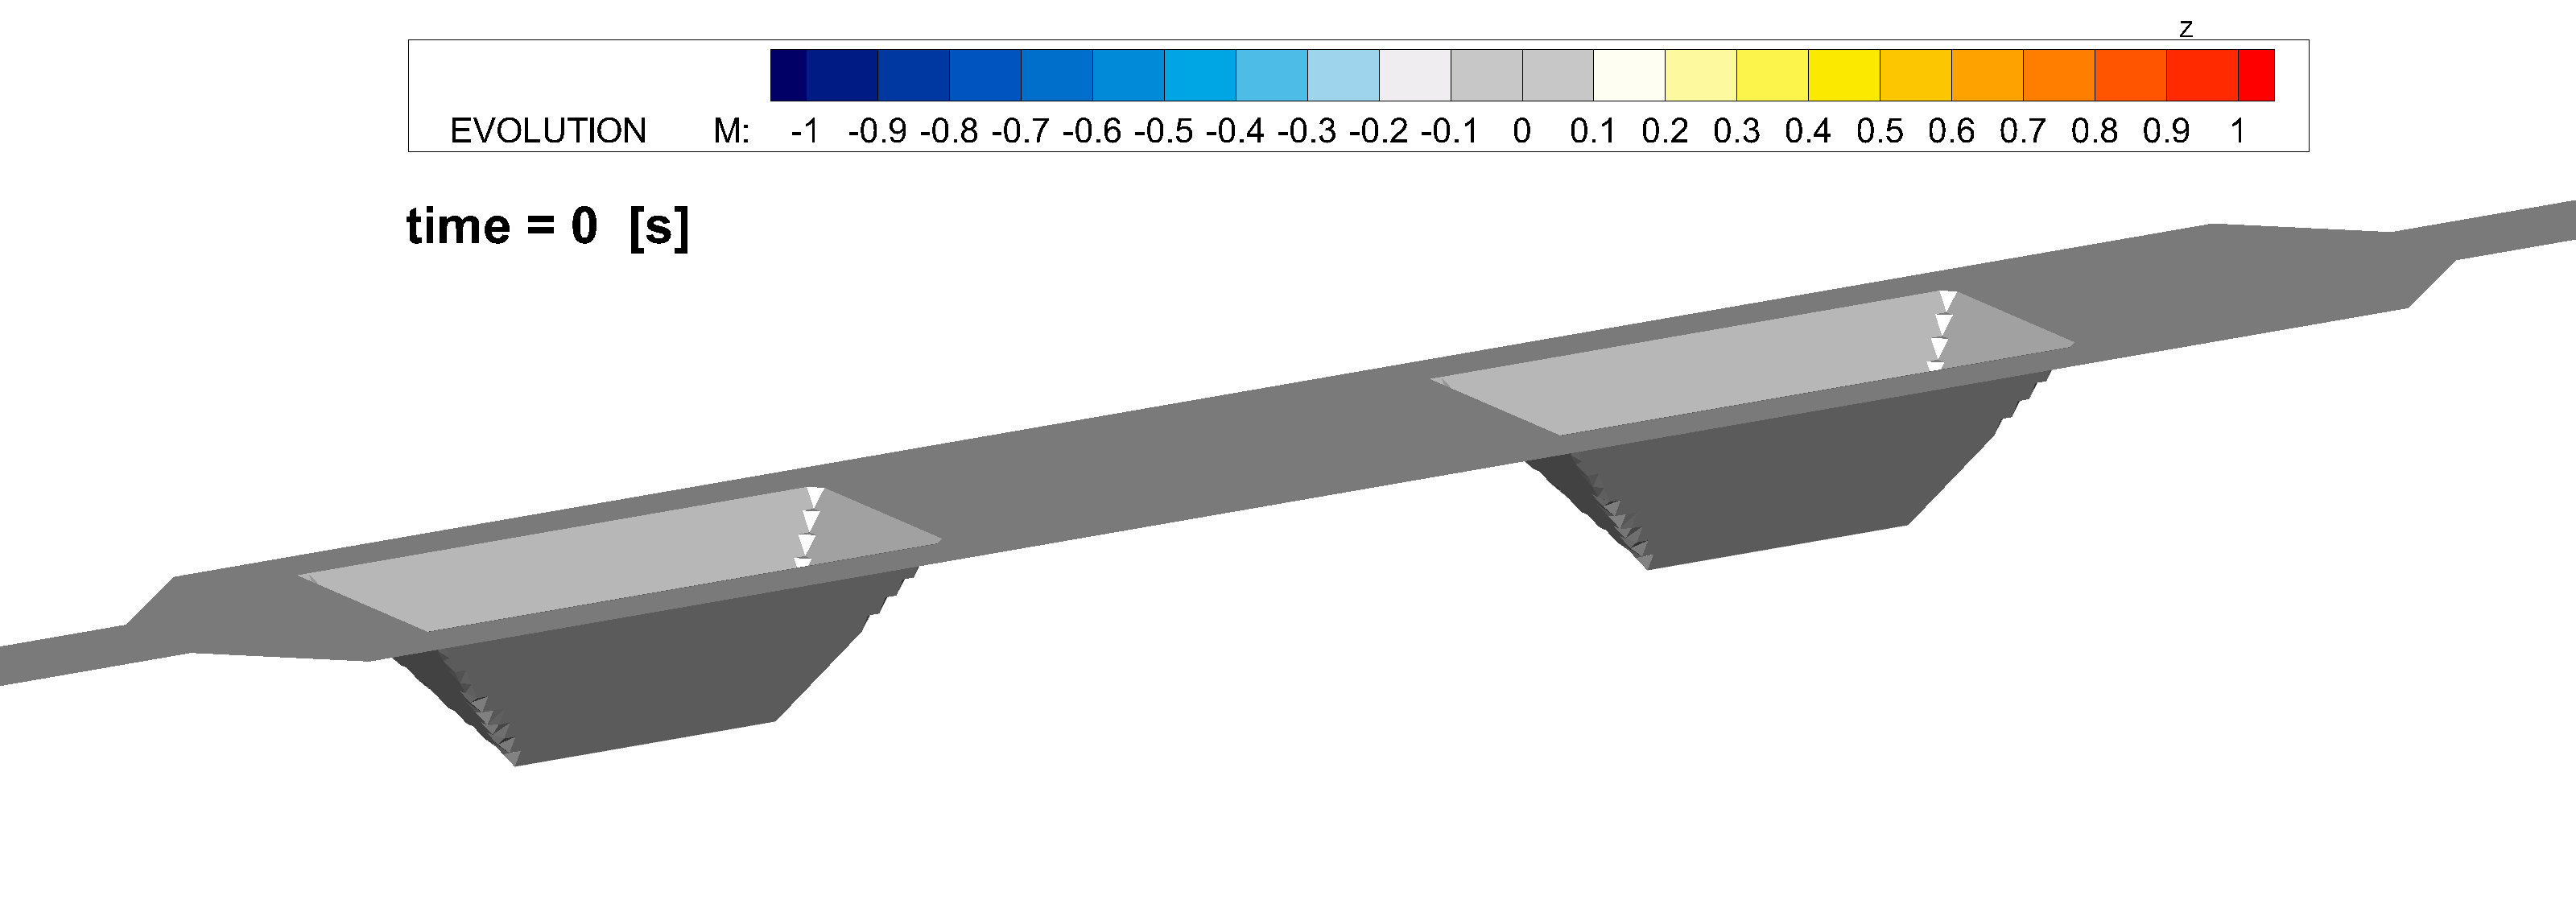
\includegraphics[scale=0.14]{result000_zoom3D.png}
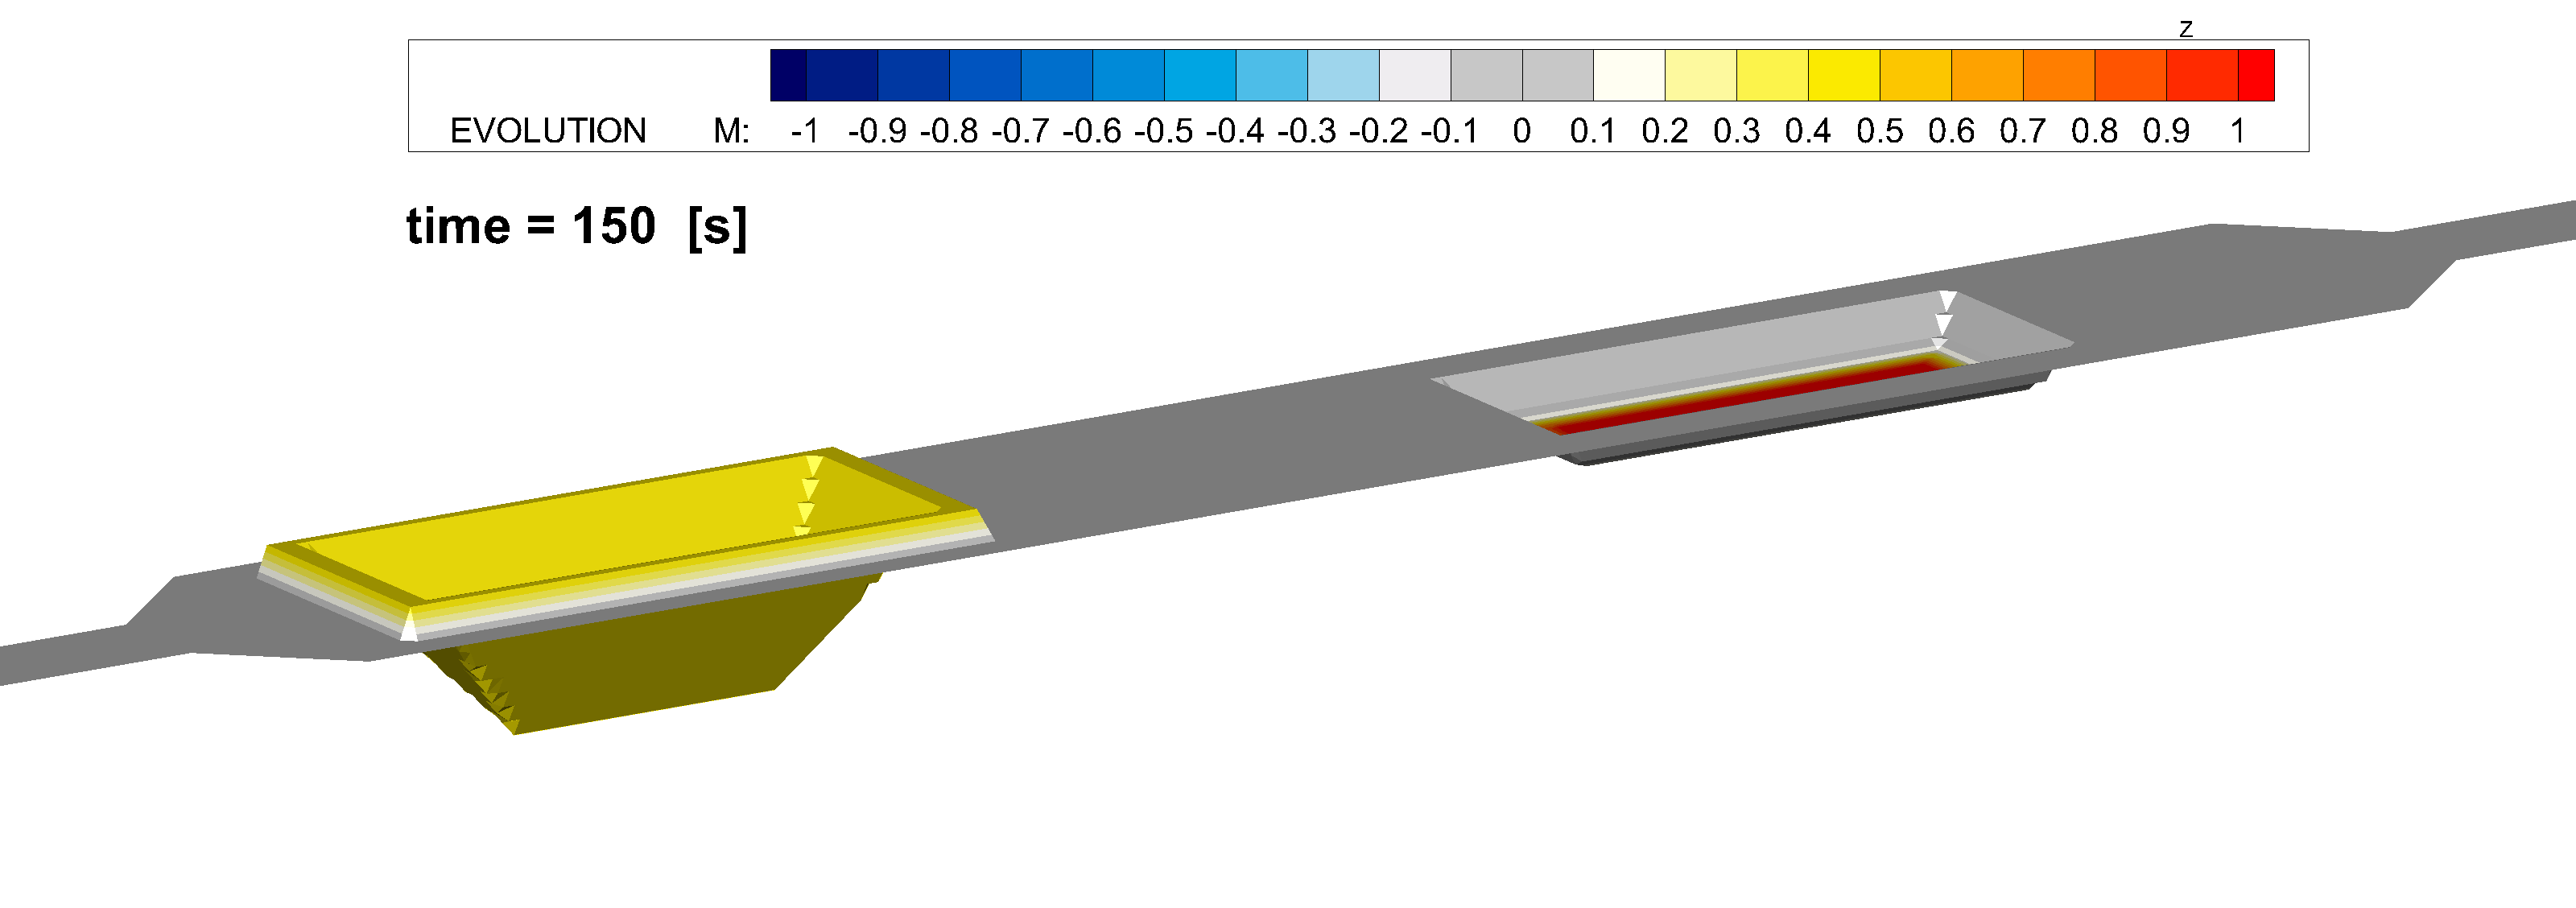
\includegraphics[scale=0.14]{result150_zoom3D.png}
\caption{Simulated evolution after 0s and 150 s.}\label{result3D}
\end{figure}


